
% !TEX encoding = UTF-8 Unicode


\documentclass{beamer}

\usetheme{Madrid}
\usepackage{graphicx}
\usepackage{epstopdf}
\DeclareGraphicsExtensions{.eps}
\usepackage{url}
\usepackage{multicol}% http://ctan.org/pkg/multicols



\usepackage{graphicx}
\usepackage{epstopdf}
\DeclareGraphicsExtensions{.eps}
\usepackage{url}
\usepackage{multicol}% http://ctan.org/pkg/multicols


  \usepackage{cite}




\usepackage[utf8x]{inputenc} 


\usepackage{array}
\newcolumntype{L}[1]{>{\raggedright\let\newline\\\arraybackslash\hspace{0pt}}m{#1}}
\newcolumntype{C}[1]{>{\centering\let\newline\\\arraybackslash\hspace{0pt}}m{#1}}
\newcolumntype{R}[1]{>{\raggedleft\let\newline\\\arraybackslash\hspace{0pt}}m{#1}}

\usepackage{float}

\usepackage{siunitx}
\usepackage{amsmath}
\usepackage{amsfonts}
\usepackage{amssymb}

\usepackage[utf8]{inputenc}

\title{Introdução ao NAS Parallel Benchmarks}

\subtitle{Performance Relativa de Kernels Sequenciais, em ambiente de Memória Partilhada e ambiente de Memória Distribuída}
% A subtitle is optional and this may be deleted

           
\author{ Filipe Costa Oliveira}


\institute[Universidade of Minho] % (optional, but mostly needed)
{
  UCE: Engenharia de Sistemas de Computação \\ 
  Mestrado Integrado em Engenharia Informática\\
  Departamento de Informática
 }


\date{Universidade do Minho, 2016}

\begin{document}

\begin{frame}
  \titlepage
\end{frame}


\begin{frame}{Introdução -- Contextualização das Benchmarks}

As "NAS Parallel Benchmarks" englobam 5 kernels (EP, MG, CG, FT, IS) e 3 aplicações  que simulam dinâmica de fluídos (LU,SP,BT). Temos por interesse os 5 kernels:

\begin{itemize}

\item \textbf{EP}: implicitamente embaraçosamente paralelo. ( espectável obtermos os melhores resultados de performance neste kernel )

\item \textbf{MG}: implica uma elevada comunicação para a resolução do algoritmo. 

\item \textbf{CG}:  testa computação e comunicação não estruturada, sendo portanto expectável uma fraca performance deste kernel quando em comparação com o \textbf{EP}. 

\item \textbf{FT}: excluído do caso de estudo em detrimento do \textbf{MG}.


\item \textbf{IS}: testa tanto a capacidade de computação de um sistema em termos de operações sobre inteiros, assim como a performance de comunicação do mesmo.

 \end{itemize}


  \end{frame}
  
  
\begin{frame}{Caracterização do Hardware do ambiente de testes e dimensão das diferentes classes de dados}

Ambiente de Clustering Search6\footnote{Services and Advanced Research Computing with HTC/HPC clusters} @ Universidade do Minho.

\begin{itemize}

\item grande porção dos nós de computação com configurações de hardware relativamente homogéneas \footnote{p.e. mesma família de processadores - Ivy Bridge} \textbf{(28 dos 54 nós disponíveis)}

\item inclusão de nós do tipo 662, 652, 641, e 431 \textbf{(abrangendo 33 dos 54 nós disponíveis)}.
\begin{itemize}

\item preservam características entre eles fundamentais para a possibilidade de comparação (p.e. suporte da rede Myrinet 10Gbps).

\item englobam como requerido mais do que uma classe de arquitectura existente no Search6.
 \end{itemize}

 \end{itemize}

{  \tiny

\begin{table}[h!]
\caption{Dimensão do dataset para as diferentes Classes e Benchmarks}
     \label{table:dimensaoproblema}
\centering
  \begin{tabular}{ | l | r |  r | r | r | r |  }
    \hline
    Bench. & data type & S & A & B & C \\ \hline 
    
     EP &  double & 128	MB & 2	GB	 & 8	GB	& 32	GB \\ \hline 
     
  MG &  double &   256	KB & 128	MB	& 128	MB	& 1024	MB \\ \hline 
    CG & double & 15MB & 1,46	GB& 41,91	GB	& 167,64	GB \\ \hline 
    IS & integer & 256	KB & 32	MB	& 128	MB	& 512	MB \\ \hline 

  \end{tabular}
\end{table}
}
  \end{frame}
  
  \begin{frame}{Caracterização do Software do ambiente de testes}

Influência de:
\begin{itemize}

\item Diferentes ferramentas de compilação (\textbf{GCC compiler suite}	e o \textbf{ Intel compilers suite}):
\begin{itemize}
\item icc versão 13.0.1 (gcc version 4.4.6 compatibility)
\item gcc versão 4.4.6
\item gcc versão  4.9.0  (versão default no nosso ambiente de clustering)
\item \textbf{sem otimização e flags de compilação -O2 e -O3 }
 \end{itemize}
 \item Diferentes configurações de ferramentas de comunicação:
 \begin{itemize}
\item Gigabit Ethernet
\item Myrinet 10Gbps
 \end{itemize}
 \item Kernels Sequenciais(SEQ), em ambiente de Memória Partilhada(OMP) e ambiente de Memória Distribuída(MPI)

 \end{itemize}


  \end{frame}
  
   \begin{frame}{Benchmarking em ambiente sequencial -- NPB SEQ}
\begin{itemize}
\item \small Kernels compilados com o compilador gcc versão 4.9.0 com flag de compilação -03 obtiveram os melhores resultados;
\item \small Máximo de Milhões de FP Operations alcançado para o kernel SEQ - MG, classe de dados C,  para  compilador gcc v4.9.0 com flag de compilação -03.
\item \small Nós do tipo compute-662 obtiveram os valores mais baixos de FP Operations por segundo \tiny{ \color{red} (figura \ref{mops_seq})}.
\item \small Compilador icc tem melhor performance nos kernels IS e EP (sem dependência de dados).
\item \small Nós do tipo compute-651 e compute-431 obtiveram os melhores valores relativamente ao tempo de computação. \tiny{ \color{red} (figura \ref{time_seq})}.
 \end{itemize}


  \end{frame}
  
   \begin{frame}{Benchmarking em ambiente sequencial -- {\small Análise FP Operations/s}}

\begin{figure}[H]
\centering
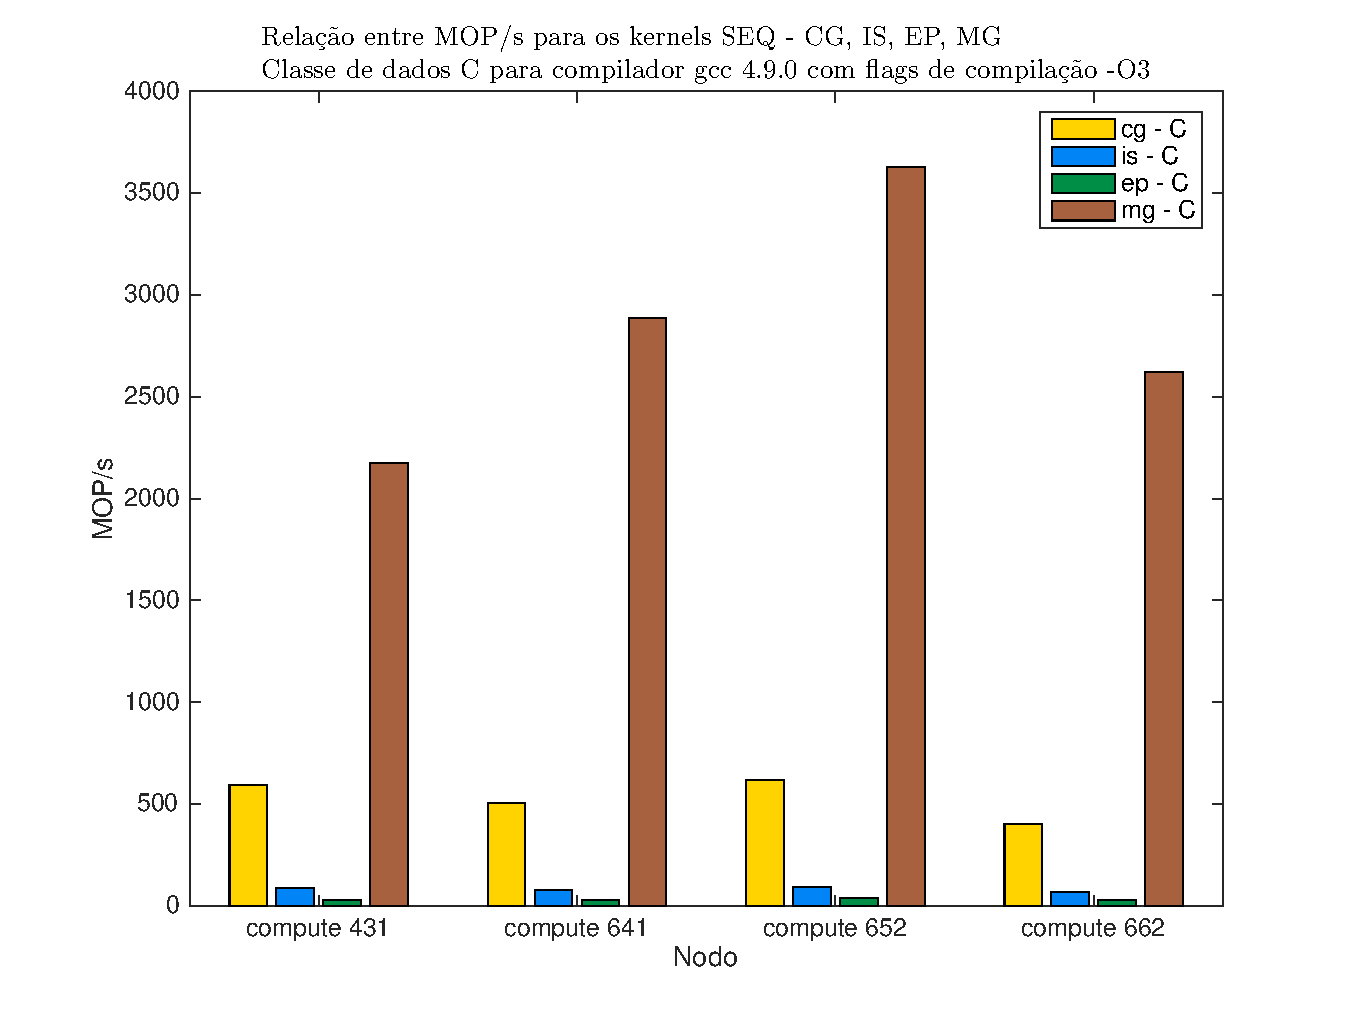
\includegraphics[width=0.75\columnwidth]{EPS/PRESENTATION_SPECIAL/mops_seq.eps}

\caption{\tiny Milhões de FP Operations alcançado para os kernels SEQ - CG, IS, EP, e MG, classe de dados C, para  compilador gcc 4.9.0 com flag de compilação -O3}
\label{mops_seq}
\end{figure}
  \end{frame}


   \begin{frame}{Benchmarking em ambiente sequencial -- {\small Análise T. Total Solução}}

\begin{figure}[H]
\centering
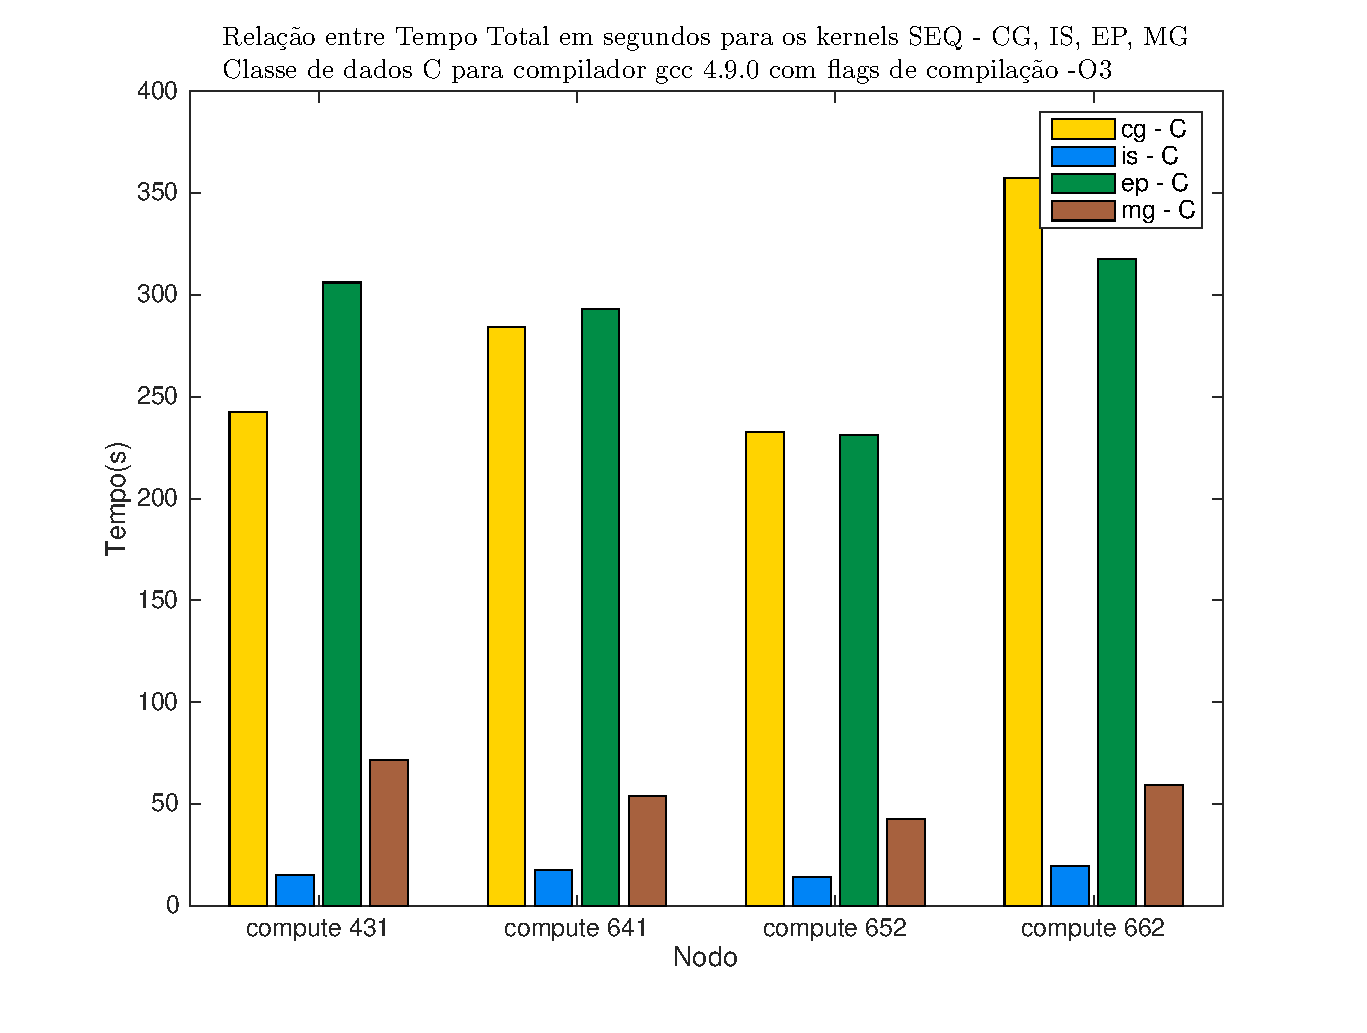
\includegraphics[width=0.75\columnwidth]{EPS/SEQ/TEMPO_seq_gcc_C_all.eps}

\caption{\tiny Milhões de FP Operations alcançado para os kernels SEQ - CG, IS, EP, e MG, classe de dados C, para  compilador gcc 4.9.0 com flag de compilação -O3}
\label{time_seq}
\end{figure}
\end{frame}


\begin{frame}{Benchmarking em Amb. de Memória Partilhada  -- NPB OMP}
\begin{itemize}
\item \small Criados casos de teste que superassem o número de threads possíveis de correrem concorrente por tipo de CPU.
\item \small Tempo total p/solução apresenta uma redução para todo os incrementes no número de threads presente na solução até ao número de threads openMP superar o número de threads disponíveis por CPU.
\item \small Nós do tipo compute-662 obtiveram os melhores valores relativamente ao tempo total para solução \tiny{ \color{red} (maior \#threads)}.
\item \small Nós do tipo compute-662 obtiveram a maior relação de ganho vs SEQ. \tiny{ \color{red} (maior \#threads e fraco resultado SEQ)}.
\begin{itemize}
\item kernel EP apresenta melhor resultado (aprox 32)
\item kernel MG apresenta melhor resultado (aprox 7)

\end{itemize}
\item \small Estudada influência de diferentes flags de compilação (-O2 / -O3) e diferentes versões de compilador (gcc 4.4.6 / gcc.4.9.0 ) para as máquinas com melhor resultado OMP (nós compute-662).


 \end{itemize}
  \end{frame}
  
     \begin{frame}{Benchmarking Amb. Mem. Partilhada  - {\small Relação de Ganho - EP}}

\begin{figure}[H]
\centering
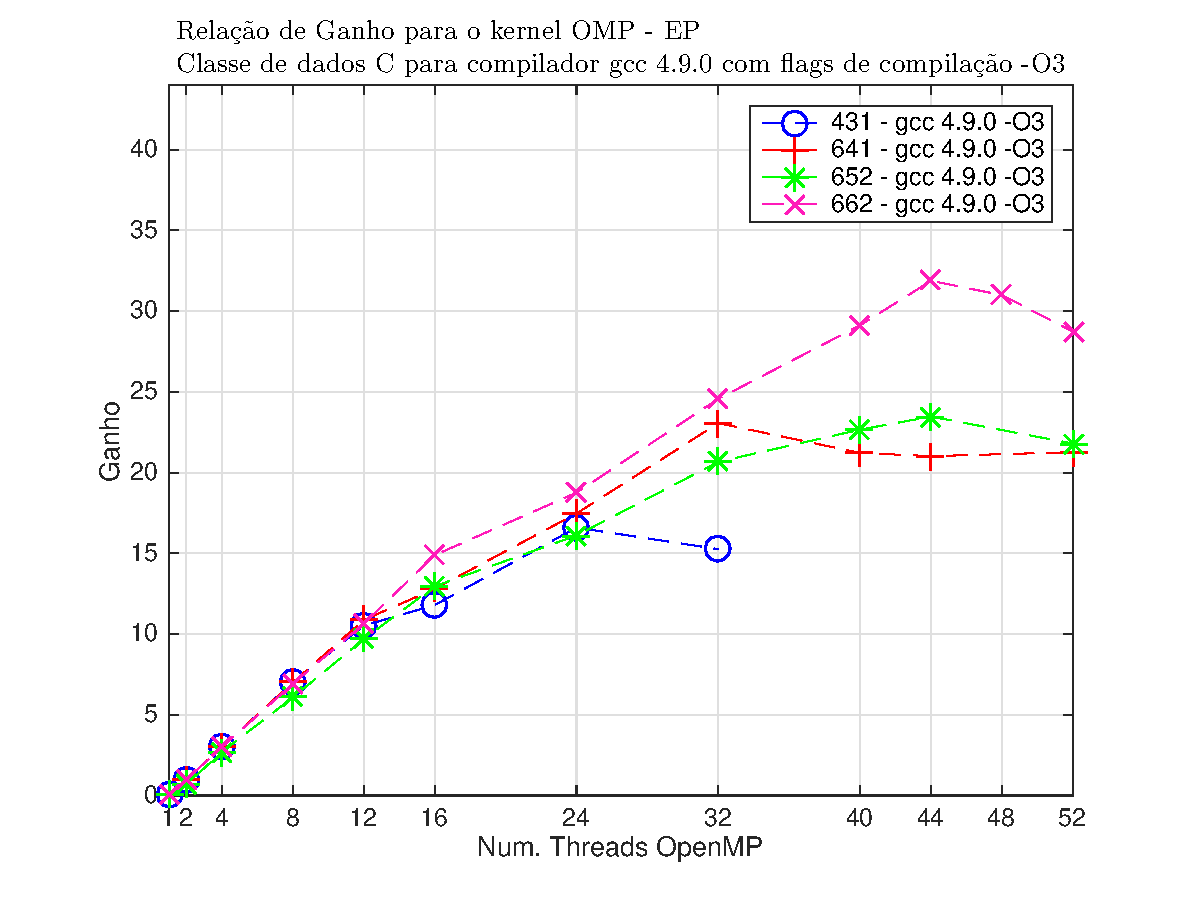
\includegraphics[width=0.75\columnwidth]{EPS/OMP/ganho_ep_03.eps}
\caption{\tiny Relação de ganho para o kernel OMP - EP, classe de dados C para  compilador gcc 4.9.0 com flag de compilação -O3}
\label{ganho_omp}
\end{figure}

  \end{frame}
  
  
     \begin{frame}{Benchmarking Amb. Mem. Partilhada  - {\small Relação de Ganho - CG}}

\begin{figure}[H]
\centering
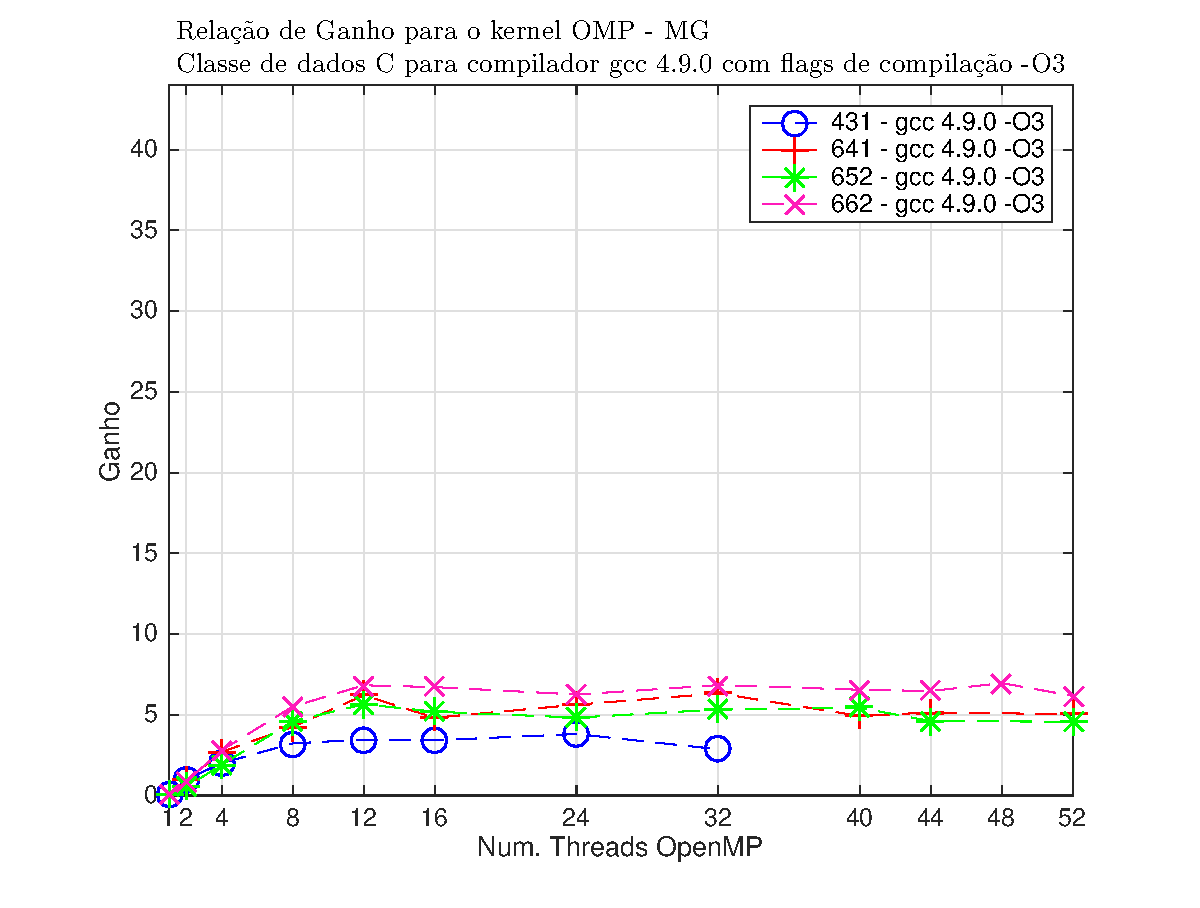
\includegraphics[width=0.75\columnwidth]{EPS/OMP/ganho_mg_03.eps}
\caption{\tiny Relação de ganho para o kernel OMP - CG, classe de dados C para  compilador gcc 4.9.0 com flag de compilação -O3}
\label{ganho_omp}
\end{figure}

  \end{frame}
  
  \begin{frame}{Benchmarking Amb. de Memória Distribuída  -- NPB MPI}
\begin{itemize}
\item \small Criados casos de teste que envolveram 2 e 4 máquinas distintas do mesmo tipo.
\begin{itemize}
\item \small 2 máquinas envolvidas na solução teremos em teste 8 e 16 processos MPI.
\item \small 4 máquinas envolvidas na solução teremos em teste 32 processos MPI.
\item \tiny (aconselhado \#processos comunicantes via Myrinet 10Gbps não ultrapassasse os 8).
\end{itemize}
\item \small Testadas diferentes formas de comunicação ( Gigabit Ethernet e Myrinet 10Gbps ).
\item \small Limitado o ambiente de teste em memória distribuída aos nós do tipo compute-641 e compute-431.
\item \small Todos os kernels em estudo a adição de nós de computação e número de processos MPI envolvidos para solução \textbf{diminui o tempo de computação} quando a comunicação entre processos é feita via \textbf{Myrinet} 10Gbps. Para os casos de comunicação via \textbf{Gigabit Ethernet} o tempo de solução \textbf{piora}.
\end{itemize}
\end{frame}
  
\begin{frame}{Relação entre tempo total solução - SEQ vs OMP vs MPI }

\begin{figure}[H]
\centering
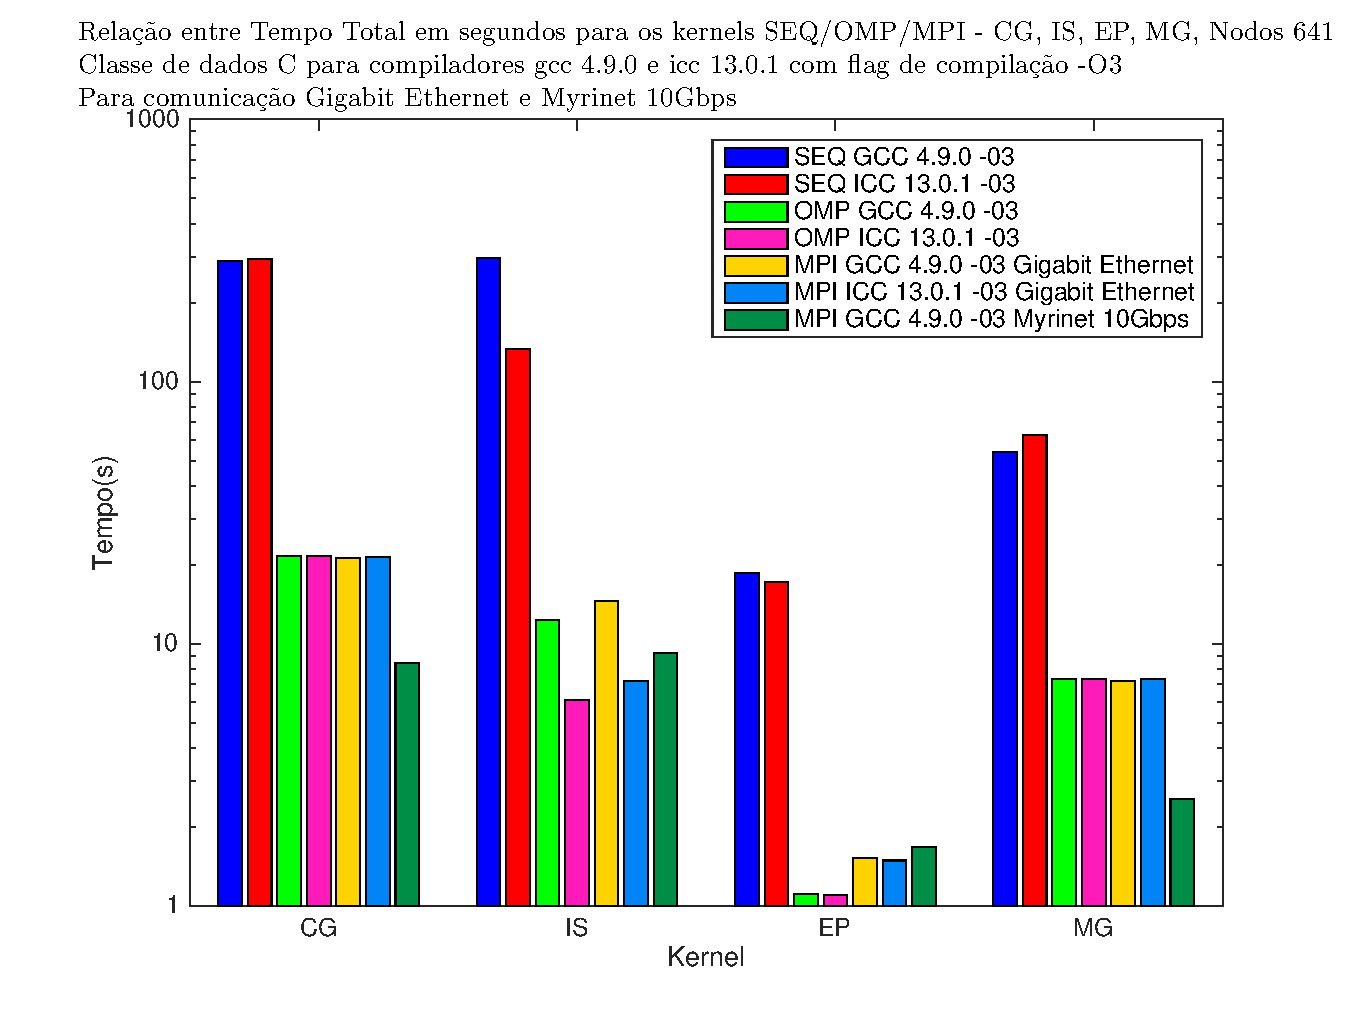
\includegraphics[width=0.75\columnwidth]{EPS/MPI/641/TIME_seq_vs_mpi_omp-gcc_vs_icc_641.eps}
\caption{\tiny Relação entre tempo total em segundos para a solução para os kernels SEQ/OMP/MPI - CG, IS, EP, MG, nós 641, classe de dados C para compiladores gcc 4.9.0 e icc 13.0.1 com flag de compilação  -O3, para comunicação Gigabit Ethernet e Myrinet 10Gbps}
\label{tempos_641}
\end{figure}

  \end{frame}
  
   \begin{frame}{Benchmarking Amb. de Memória Distribuída  -- NPB MPI}
\begin{itemize}
\item \small Kernels EP e IS a melhor solução: ambiente de memória partilhada com paralelismo via threads openMP.
\item \small Kernels CG e MG a melhor solução: ambiente de memória distribuída com comunicação via Myrinet 10Gbps.
\item \small A solução em ambiente de memória distribuída é sempre melhor com comunicação via Myrinet 10Gbps
\begin{itemize}
\item \small latência de comunicação: comunicação via Gigabit Ethernet ronda valores entre os 10 e 100 $\mu$s.
\item \small latência de comunicação: via Myrinet 10Gbps ronda valores entre os 1 e 10 $\mu$s.
\item \small Analisemos essa suposição teórica na figura \ref{ganho_omp}.
\end{itemize}
\end{itemize}
\end{frame}
\begin{frame}{\small Benchmarking Amb. Mem. Partilhada  - {\small Relação de Ganho - ETH vs MX}}

\begin{figure}[H]
\centering
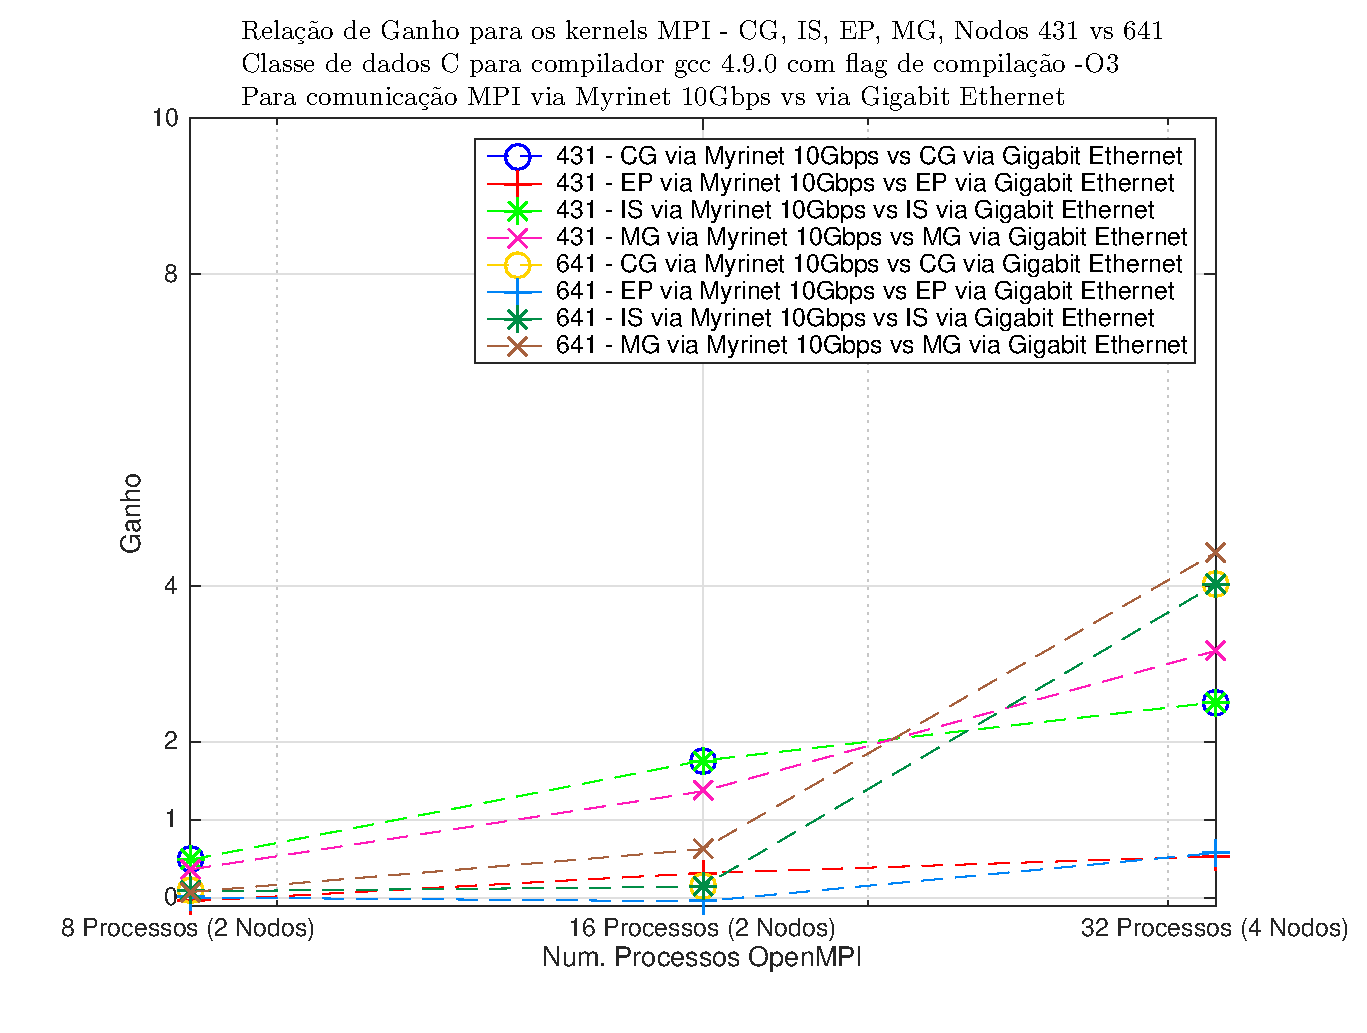
\includegraphics[width=0.75\columnwidth]{EPS/MPI/myri_vs_eth_431_vs_641.eps}
\caption{\tiny Relação de ganho para os kernels MPI - CG, IS, EP, MG, nós 431 e 641, classe de dados C para compilador gcc 4.9.0 com flag de compilação  -O3, para comunicação Gigabit Ethernet vs Myrinet 10Gbps}
\label{ganho_omp}
\end{figure}
\end{frame}

\begin{frame}{ Relação de ganho vs SEQ  -- kernels OMP e MPI }



\begin{figure}[H]
\centering
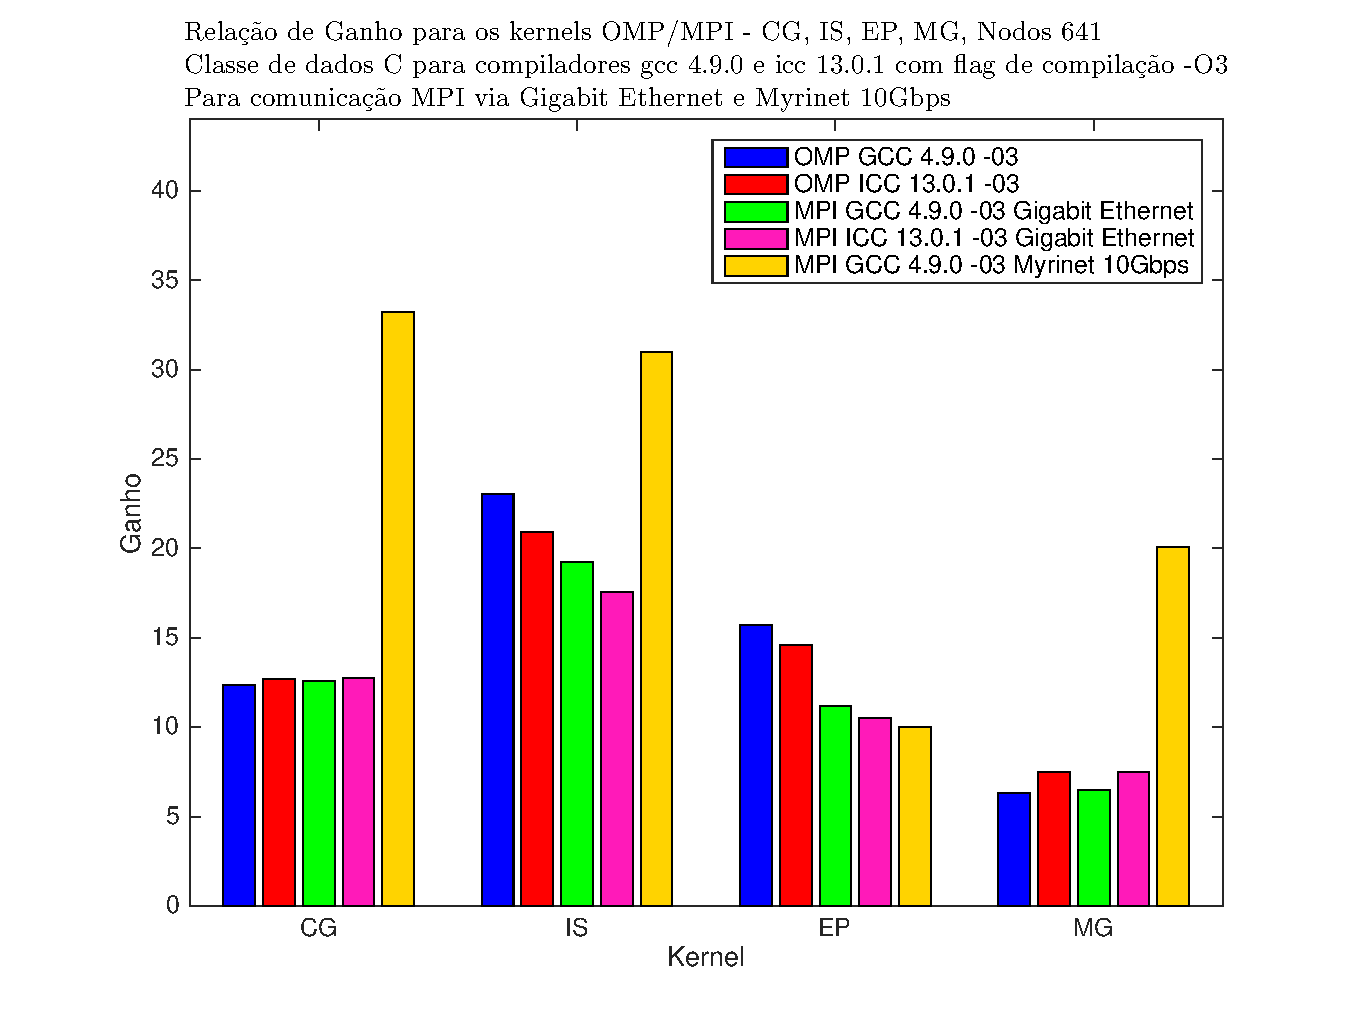
\includegraphics[width=0.75\columnwidth]{EPS/MPI/641/ganho_mpi_omp_vs_seq_641.eps}
\caption{\tiny Relação de ganho para os kernels OMP/MPI - CG, IS, EP, MG, nós 641, classe de dados C para compilador gcc 4.9.0 e icc 13.0.1 com flag de compilação  -O3, para comunicação(apenas kernels MPI) Gigabit Ethernet vs Myrinet 10Gbps}
\label{ganhos_todos_641}
\end{figure}
\end{frame}



\begin{frame}{ Relação de ganho vs SEQ  -- kernels OMP e MPI -- conclusões}
Melhores soluções do conjunto de testes realizados são:
\begin{itemize}
\item \textbf{CG} - Kernel em memória distribuída com comunicação via Myrinet 10Gbps (4 nós 32 Processos), compilador gcc 4.9.0 flag -O3;
\item \textbf{IS} - Kernel em memória partilhada com nº de processos openMP igual ao número de threads disponível, compilador gcc 4.9.0 flag -O3;
\item \textbf{EP} - Kernel em memória partilhada com nº de processos openMP igual ao número de threads disponível, compilador gcc 4.9.0 ou compilador icc 13.0.1 flag -O3;
\item \textbf{MG} - Kernel em memória distribuída com comunicação via Myrinet 10Gbps (4 nós 32 Processos), compilador gcc 4.9.0 flag -O3;

\end{itemize}
\end{frame}

\begin{frame}{ Análise de propriedades para monitorização de execução do mesmo kernel para diferentes implementações SEQ, OMP e MPI}

\begin{itemize}
\item \small As \textbf{melhores soluções} consomem quase a totalidade da capacidade de computação dos nós.
\begin{itemize}
\item \small o oposto, no nosso caso de estudo, implica que existe uma melhor solução alternativa.
\end{itemize}
\item \small Kernels com melhor solução implementada em \textbf{ambiente de memória partilhada} apresentam um maior número de \textbf{interrupções do sistema e context swap} (EP e IS).
\item \small Kernels que impliquem uma elevada comunicação para a resolução do algoritmo apresentam a melhor solução em \textbf{ambiente de memória distribuída} (CG e MG).
\item \small Nenhum dos kernels recorre intensivamente a leitura e escrita em disco por grandes períodos, centrando os mesmos ora no início ou término do mesmo.
\item \small Resultados do teste de performance mantêm-se inalterados independentemente da sequência de "n-testes" realizados.

\end{itemize}

\end{frame}


\begin{frame}{ \tiny Análise de propriedades para monitorização de execução do mesmo kernel para diferentes implementações SEQ, OMP e MPI - EP}


\begin{columns}[t]
\column{.5\textwidth}
\centering



\begin{figure}[H]
\centering
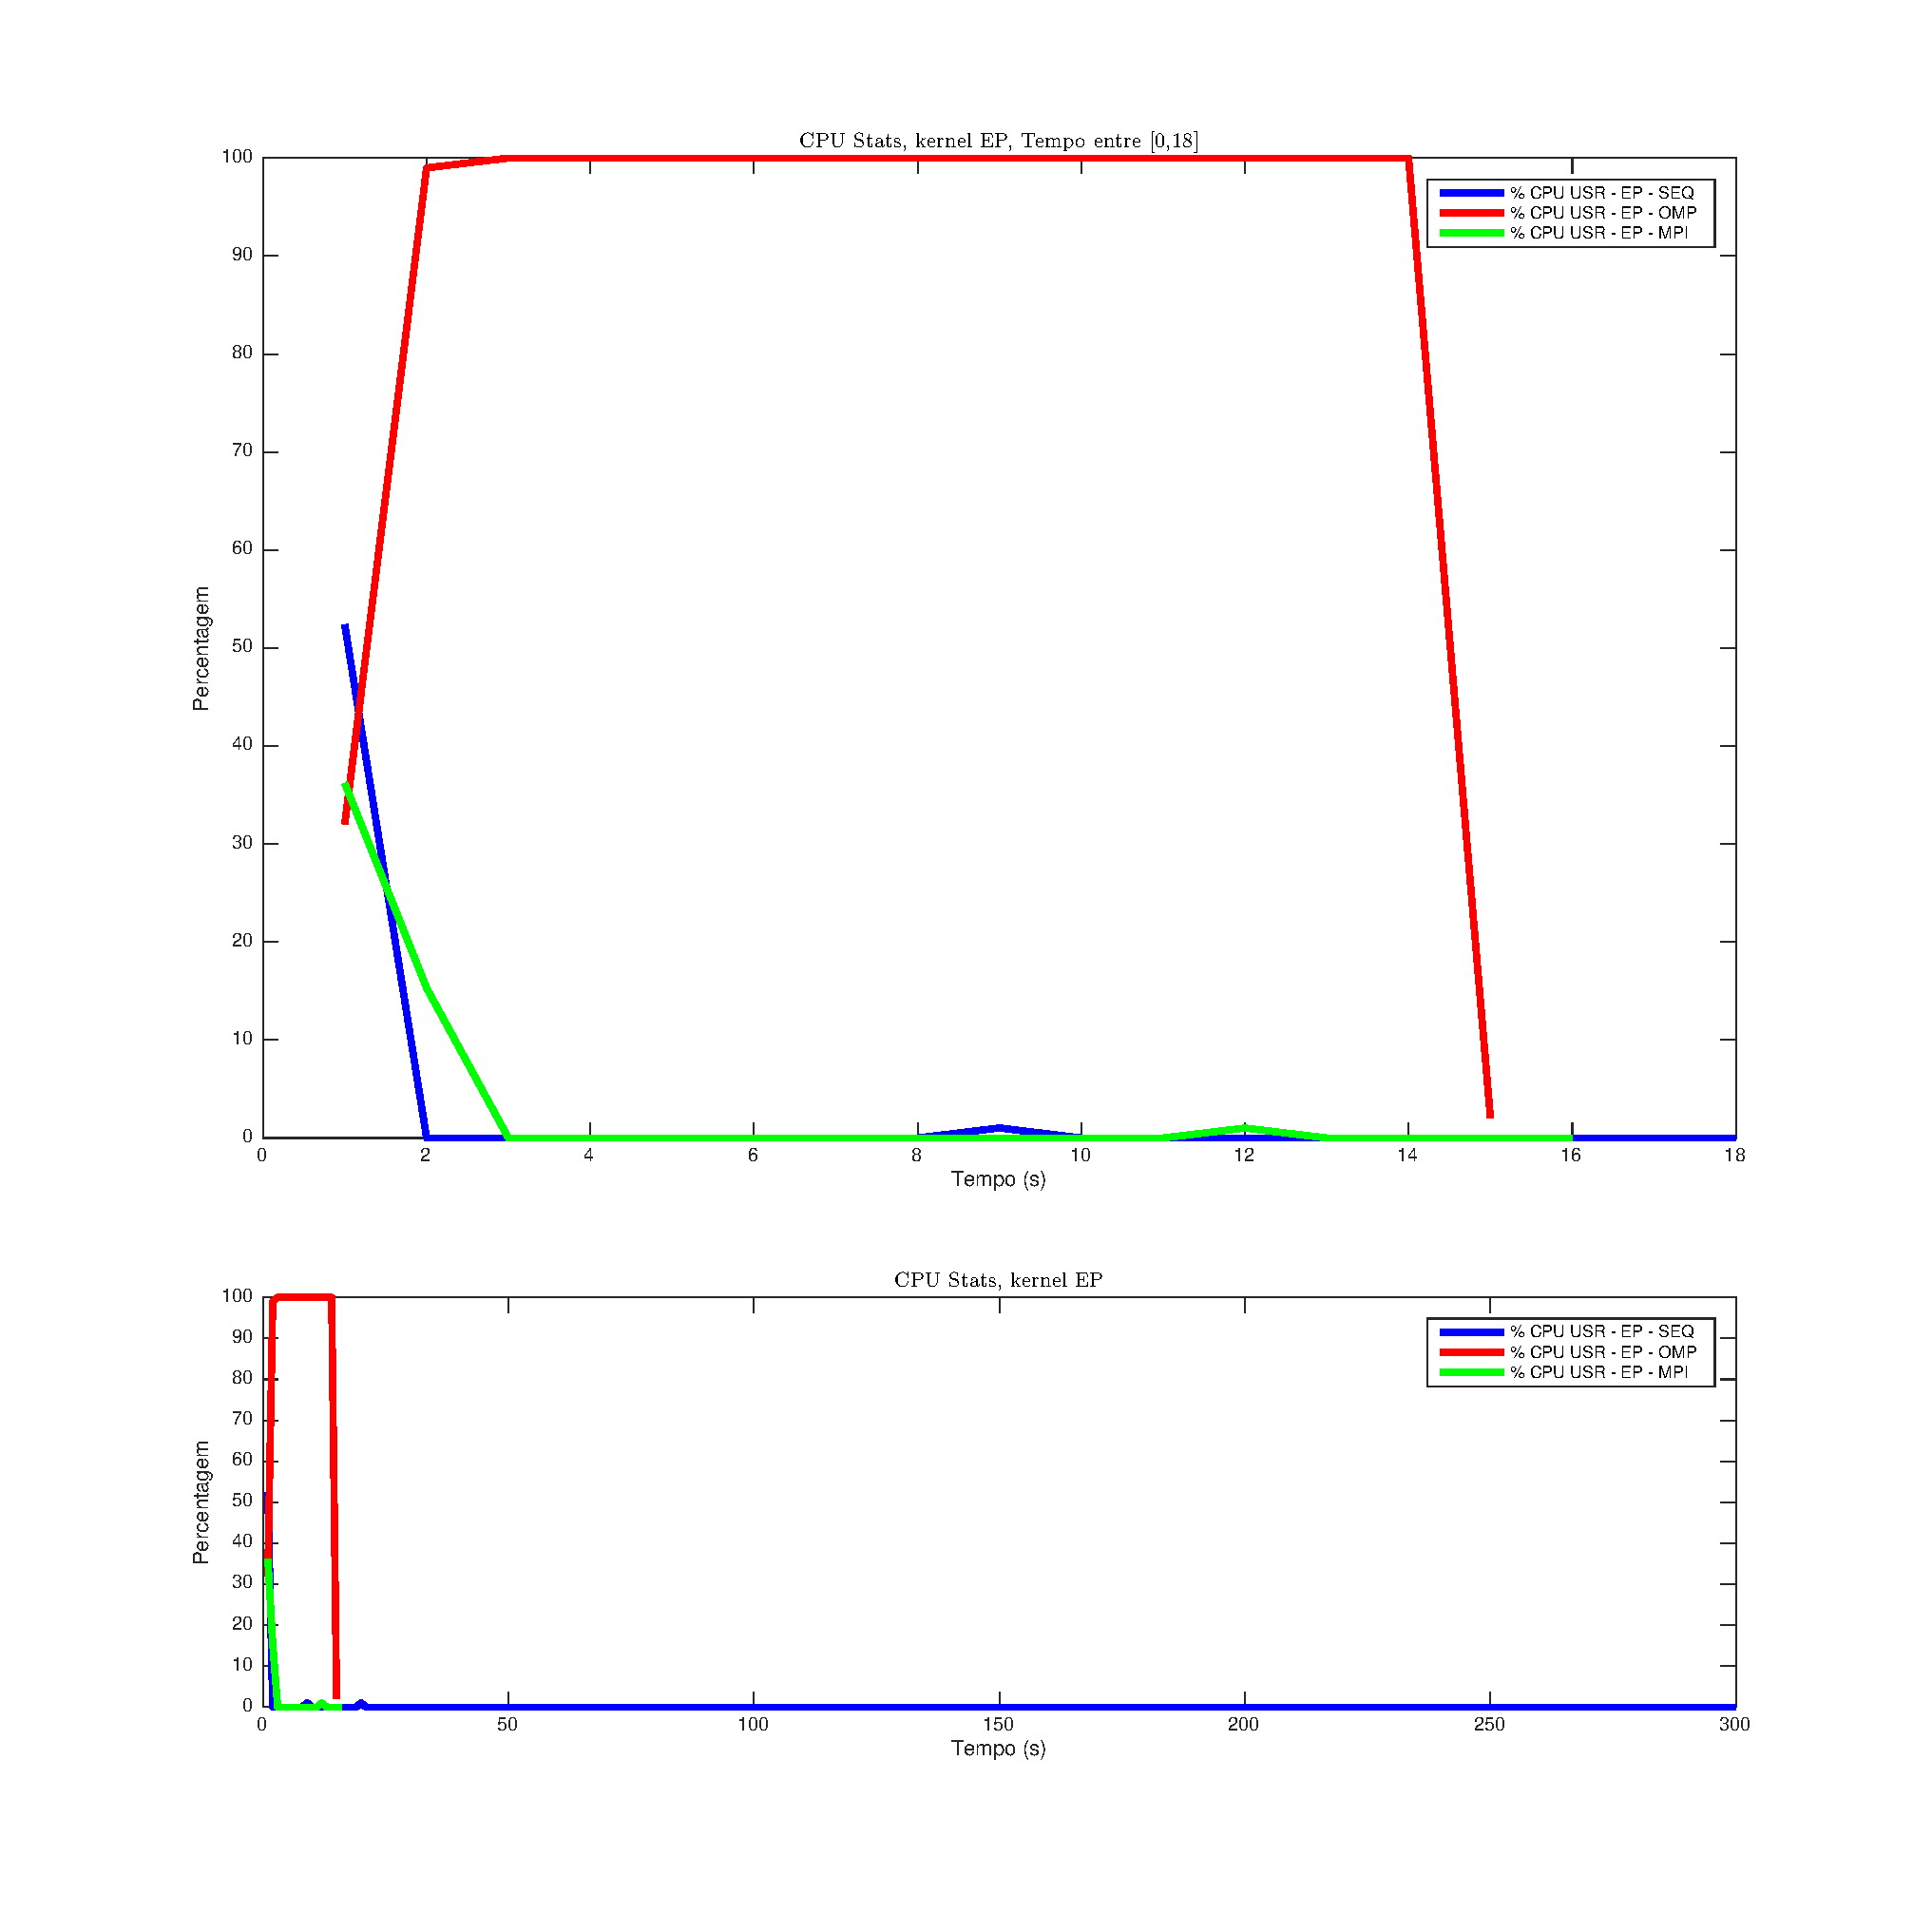
\includegraphics[width=0.9\columnwidth]{EPS/dstat_EP_seq_vs_omp_vs_mpi/cpu.eps}
\caption{\tiny Relação de \% de tempo de CPU para os kernels SEQ/OMP/MPI - EP, nós 641, classe de dados C para compilador gcc 4.9.0 com flag de compilação  -O3, para comunicação Myrinet 10Gbps (memória partilhada)}
\label{dstat_ep_SOM_cpu}
\end{figure}

\column{.5\textwidth}
\centering





\begin{figure}[H]
\centering
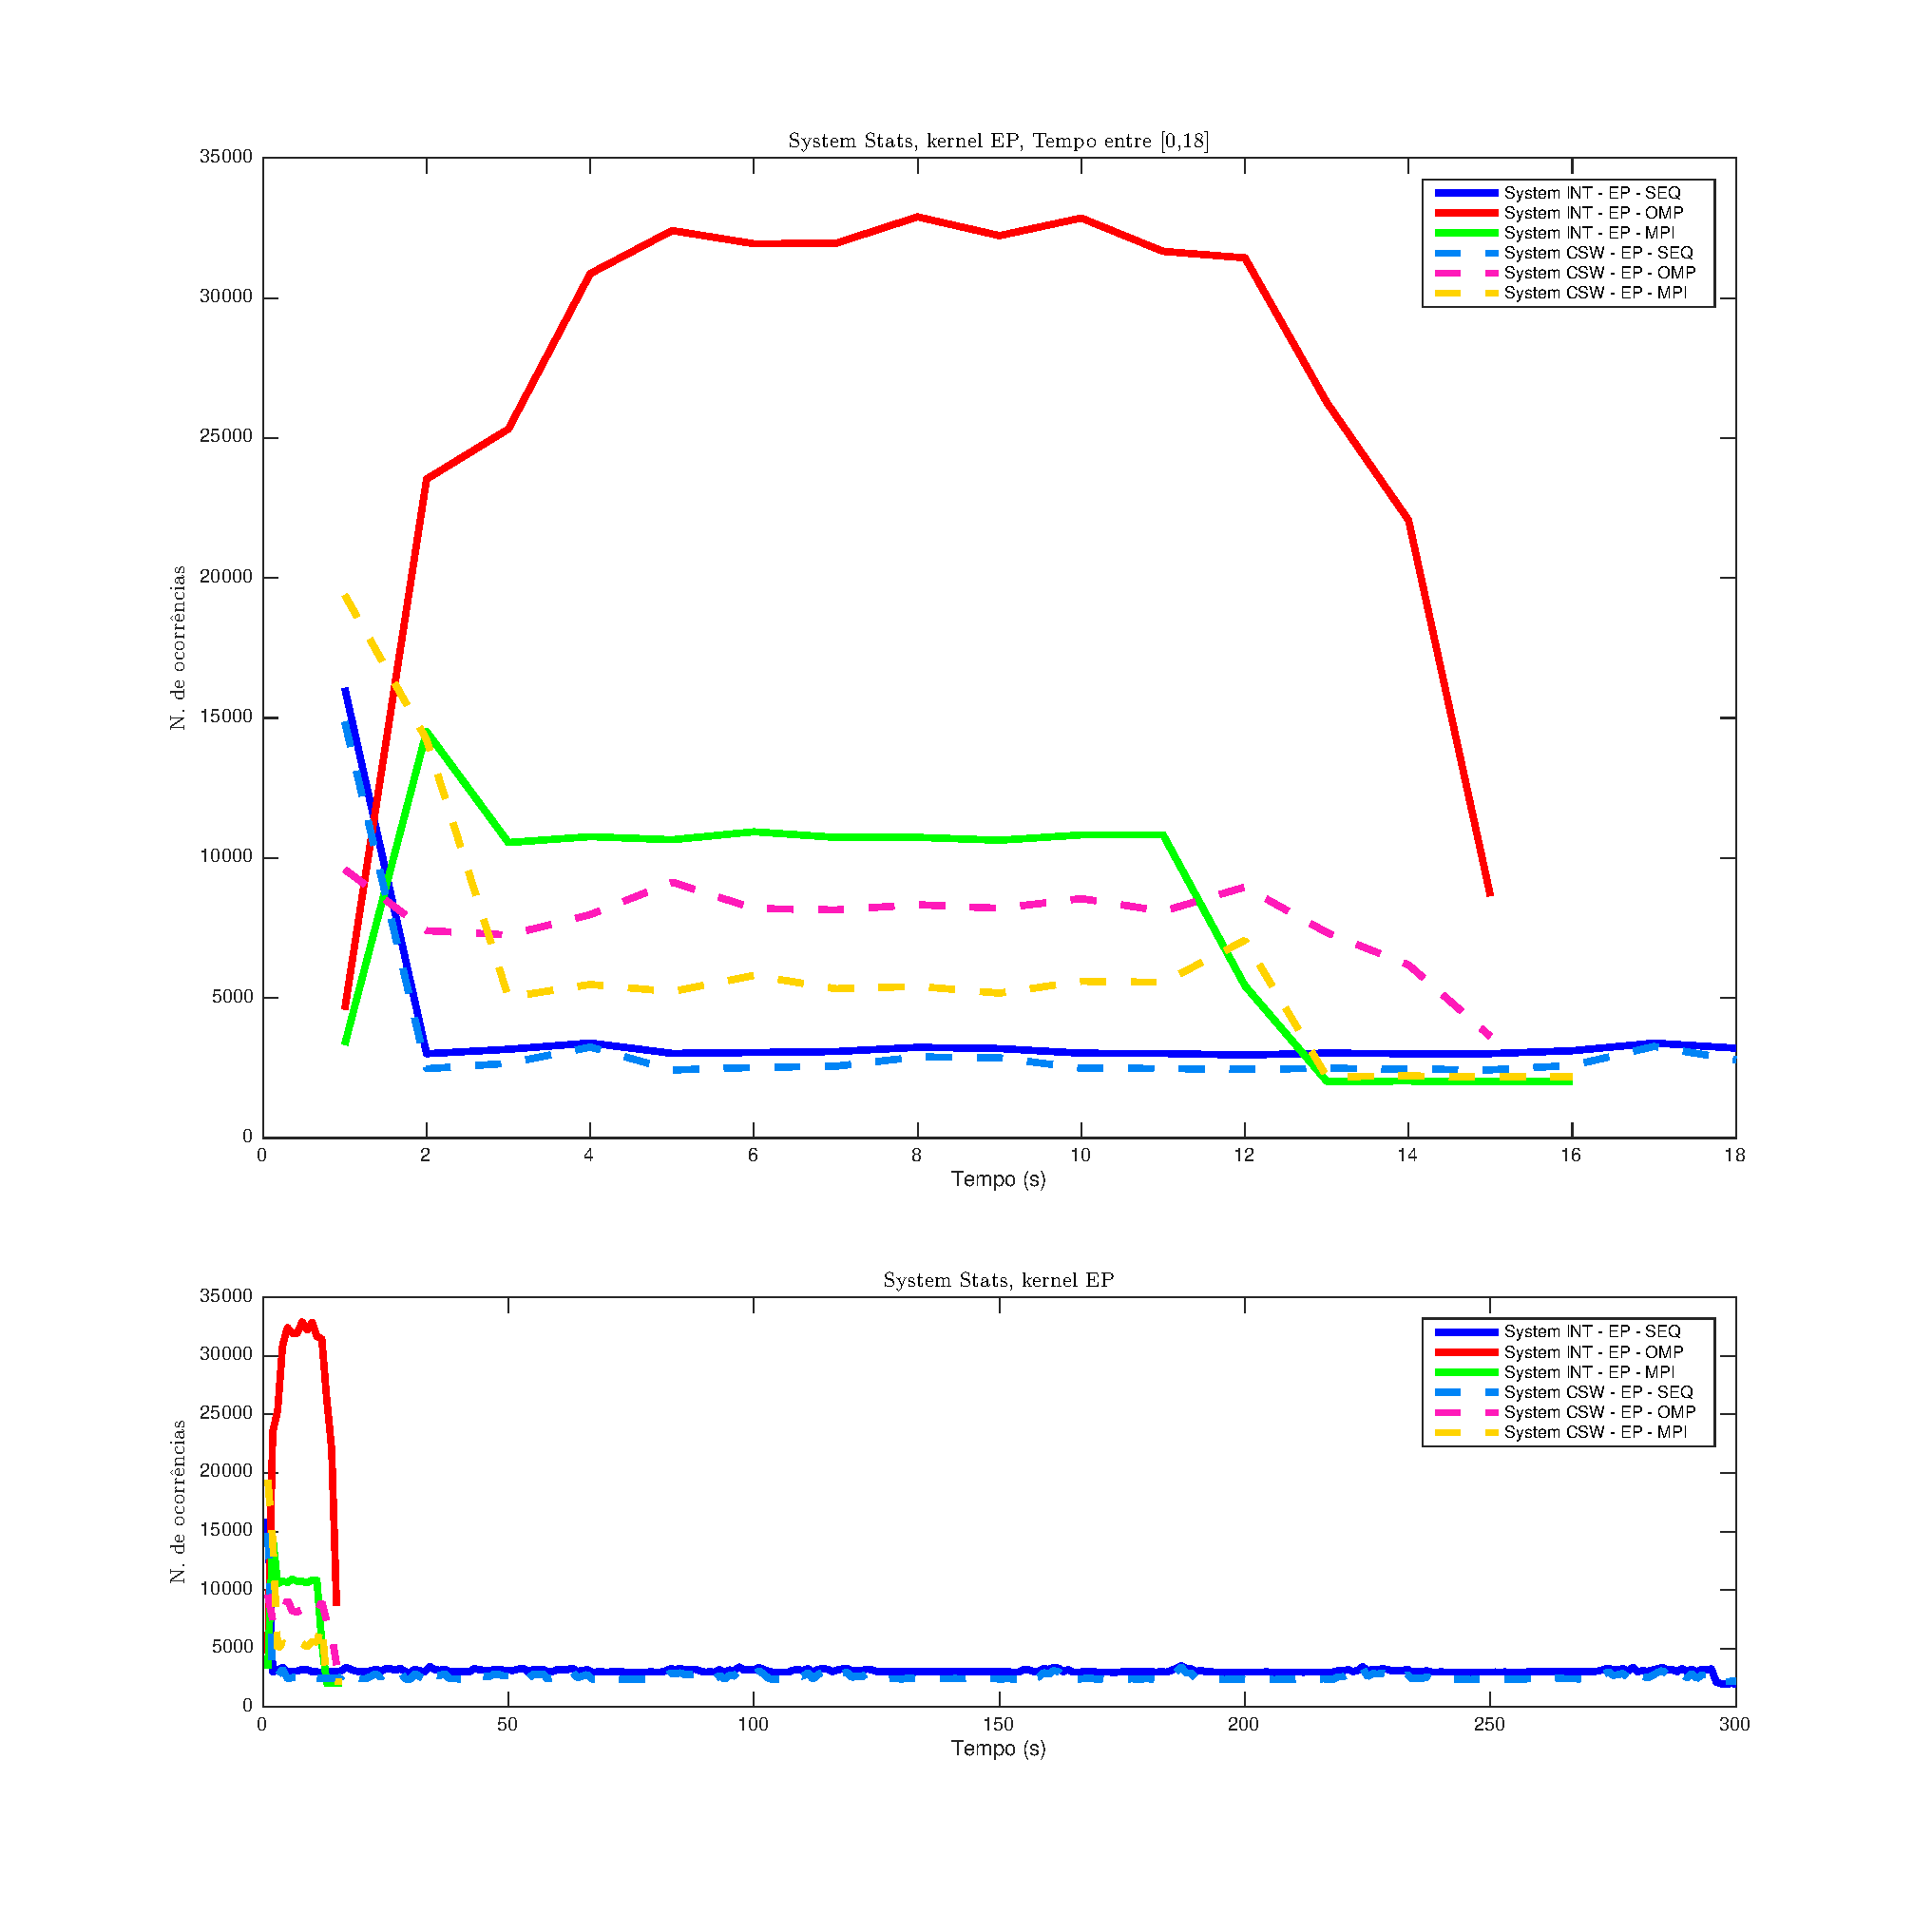
\includegraphics[width=0.9\columnwidth]{EPS/dstat_EP_seq_vs_omp_vs_mpi/system.eps}
\caption{\tiny Relação de número de interrupções de processo e número de "context swap" para os kernels SEQ/OMP/MPI - EP, nós 641, classe de dados C para compilador gcc 4.9.0 com flag de compilação  -O3, para comunicação Myrinet 10Gbps (memória partilhada)}
\label{dstat_ep_SOM_system}
\end{figure}
\end{columns}

\end{frame}


\begin{frame}{ \tiny Análise de propriedades para monitorização de execução do mesmo kernel para diferentes implementações SEQ, OMP e MPI - CG}

\begin{columns}[t]
\column{.5\textwidth}
\centering
\begin{figure}[H]
\centering
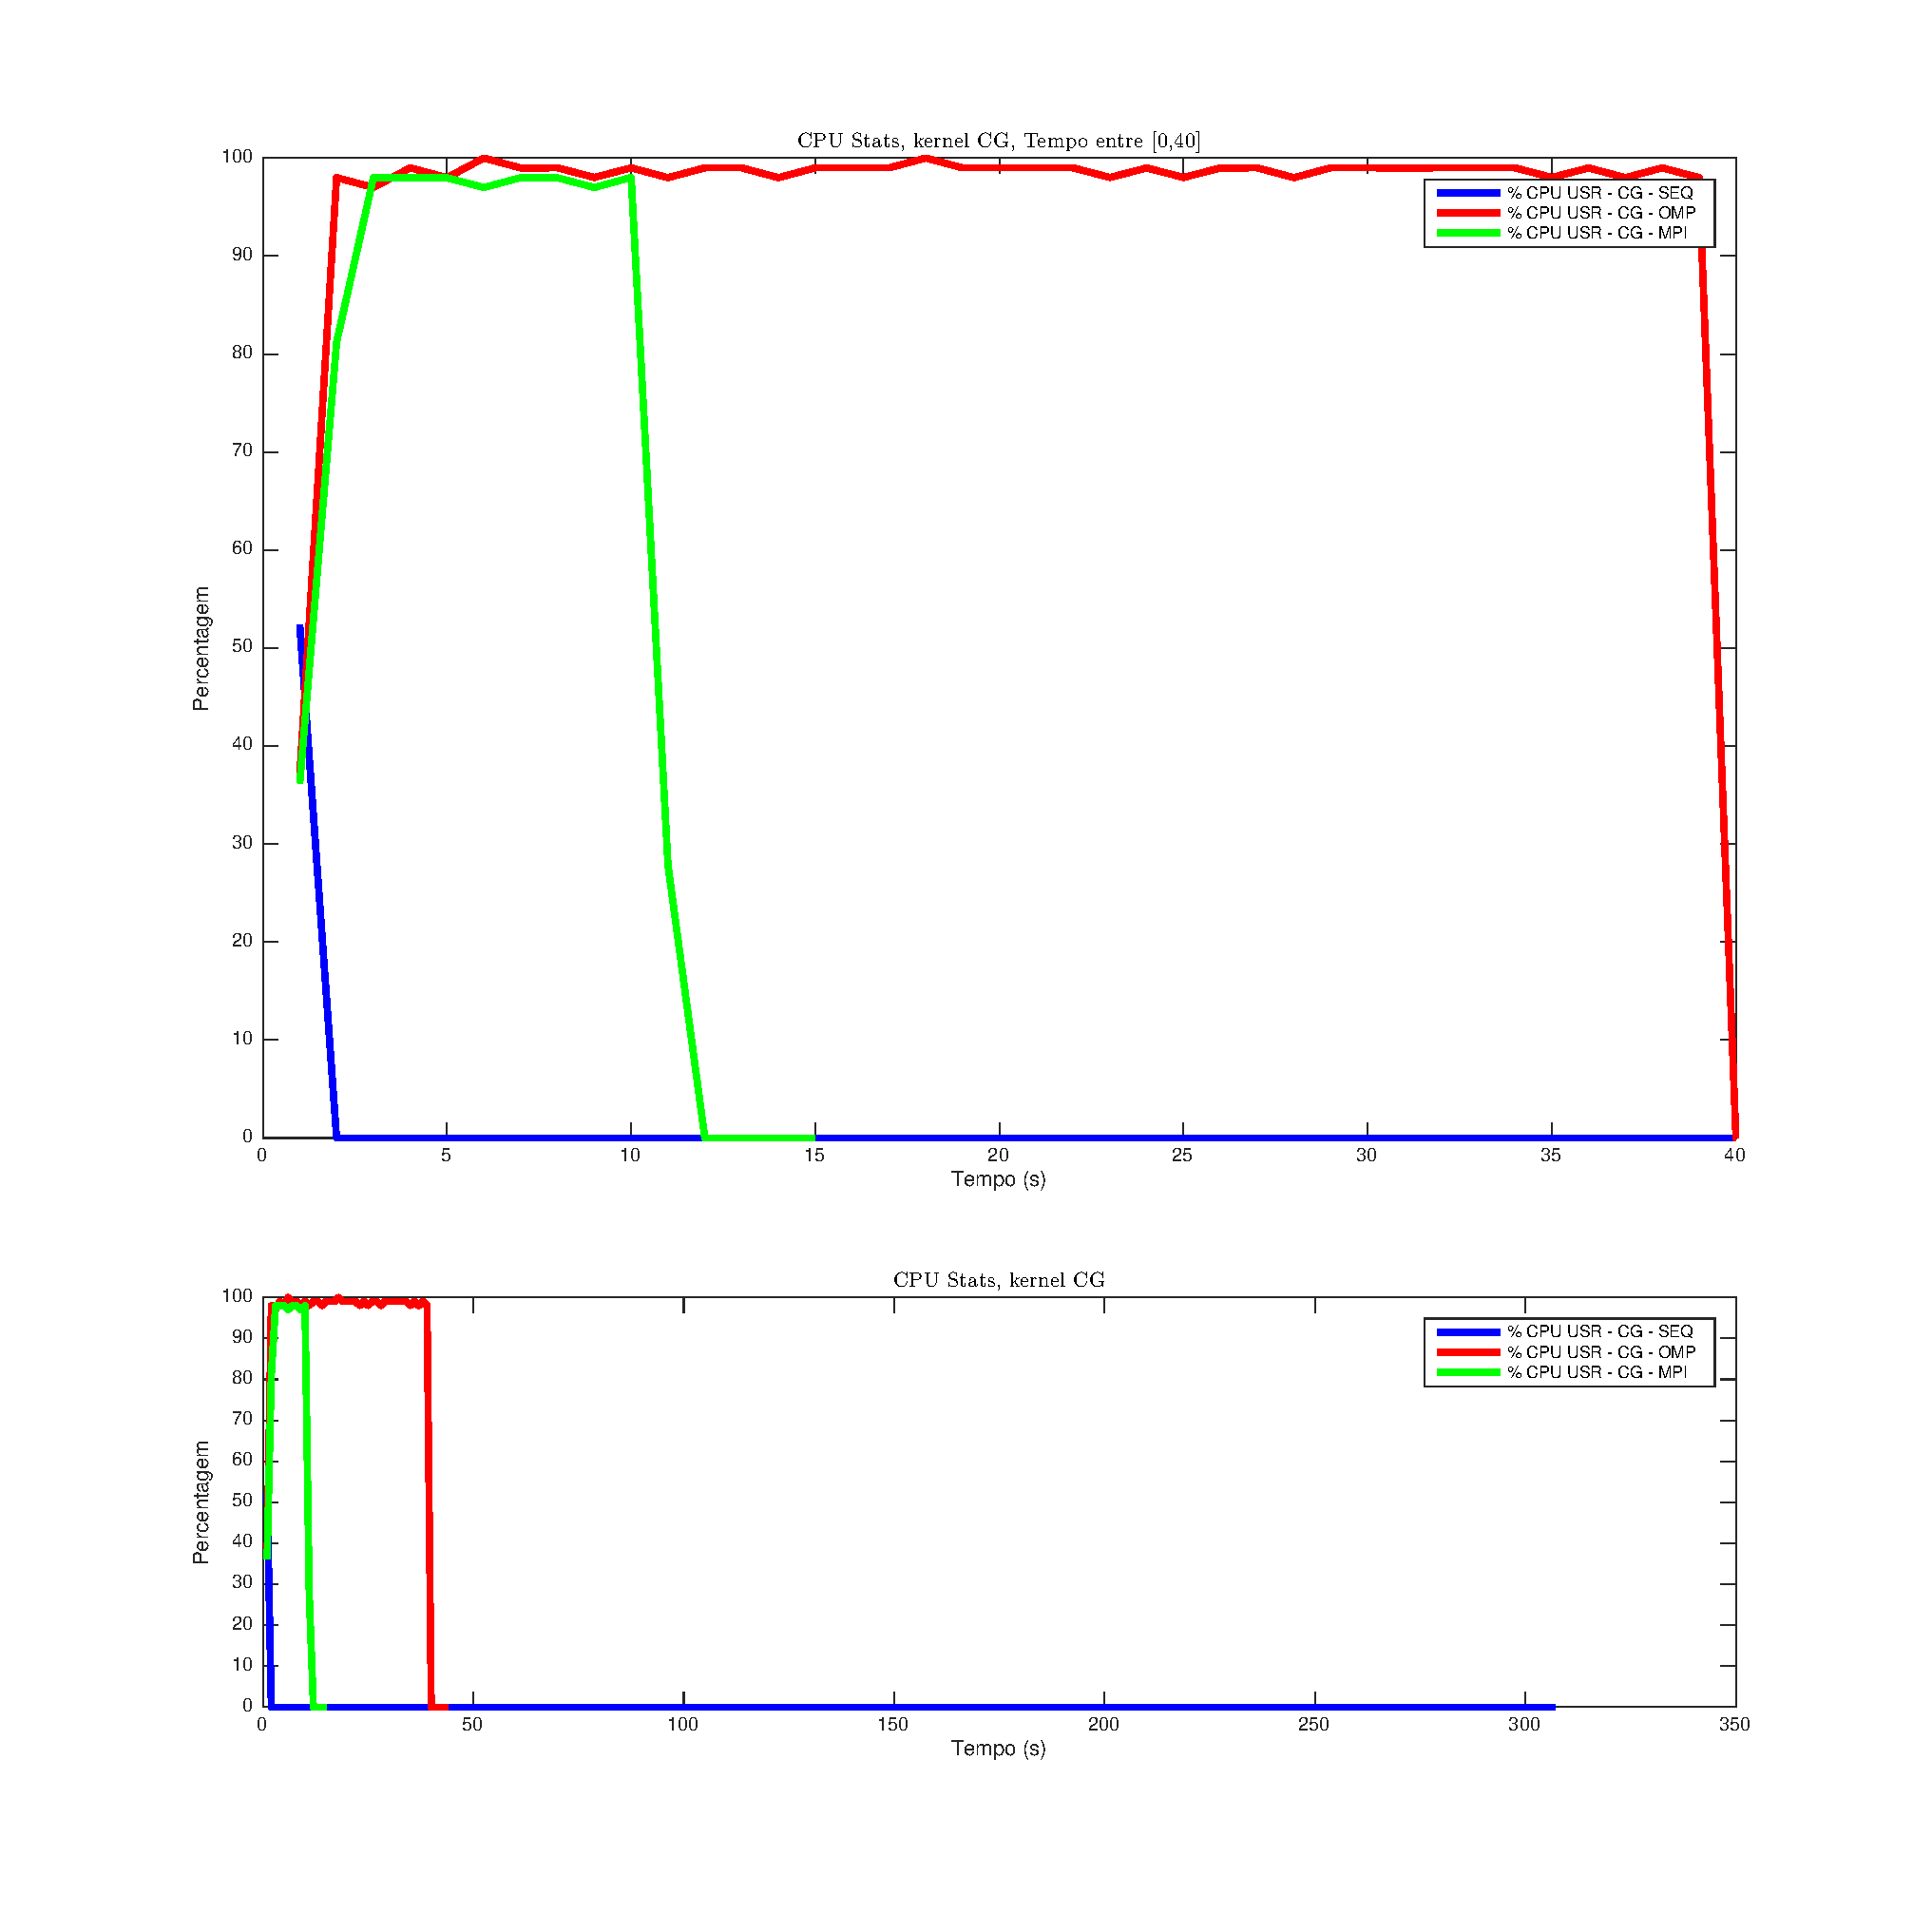
\includegraphics[width=0.9\columnwidth]{EPS/dstat_CG_seq_vs_omp_vs_mpi/cpu.eps}
\caption{\tiny  Relação de \% de tempo de CPU para os kernels SEQ/OMP/MPI - CG, nós 641, classe de dados C para compilador gcc 4.9.0 com flag de compilação  -O3, para comunicação Myrinet 10Gbps (memória distribuída)}
\label{dstat_cg_SOM_cpu}
\end{figure}

\column{.5\textwidth}
\centering
\begin{figure}[H]
\centering
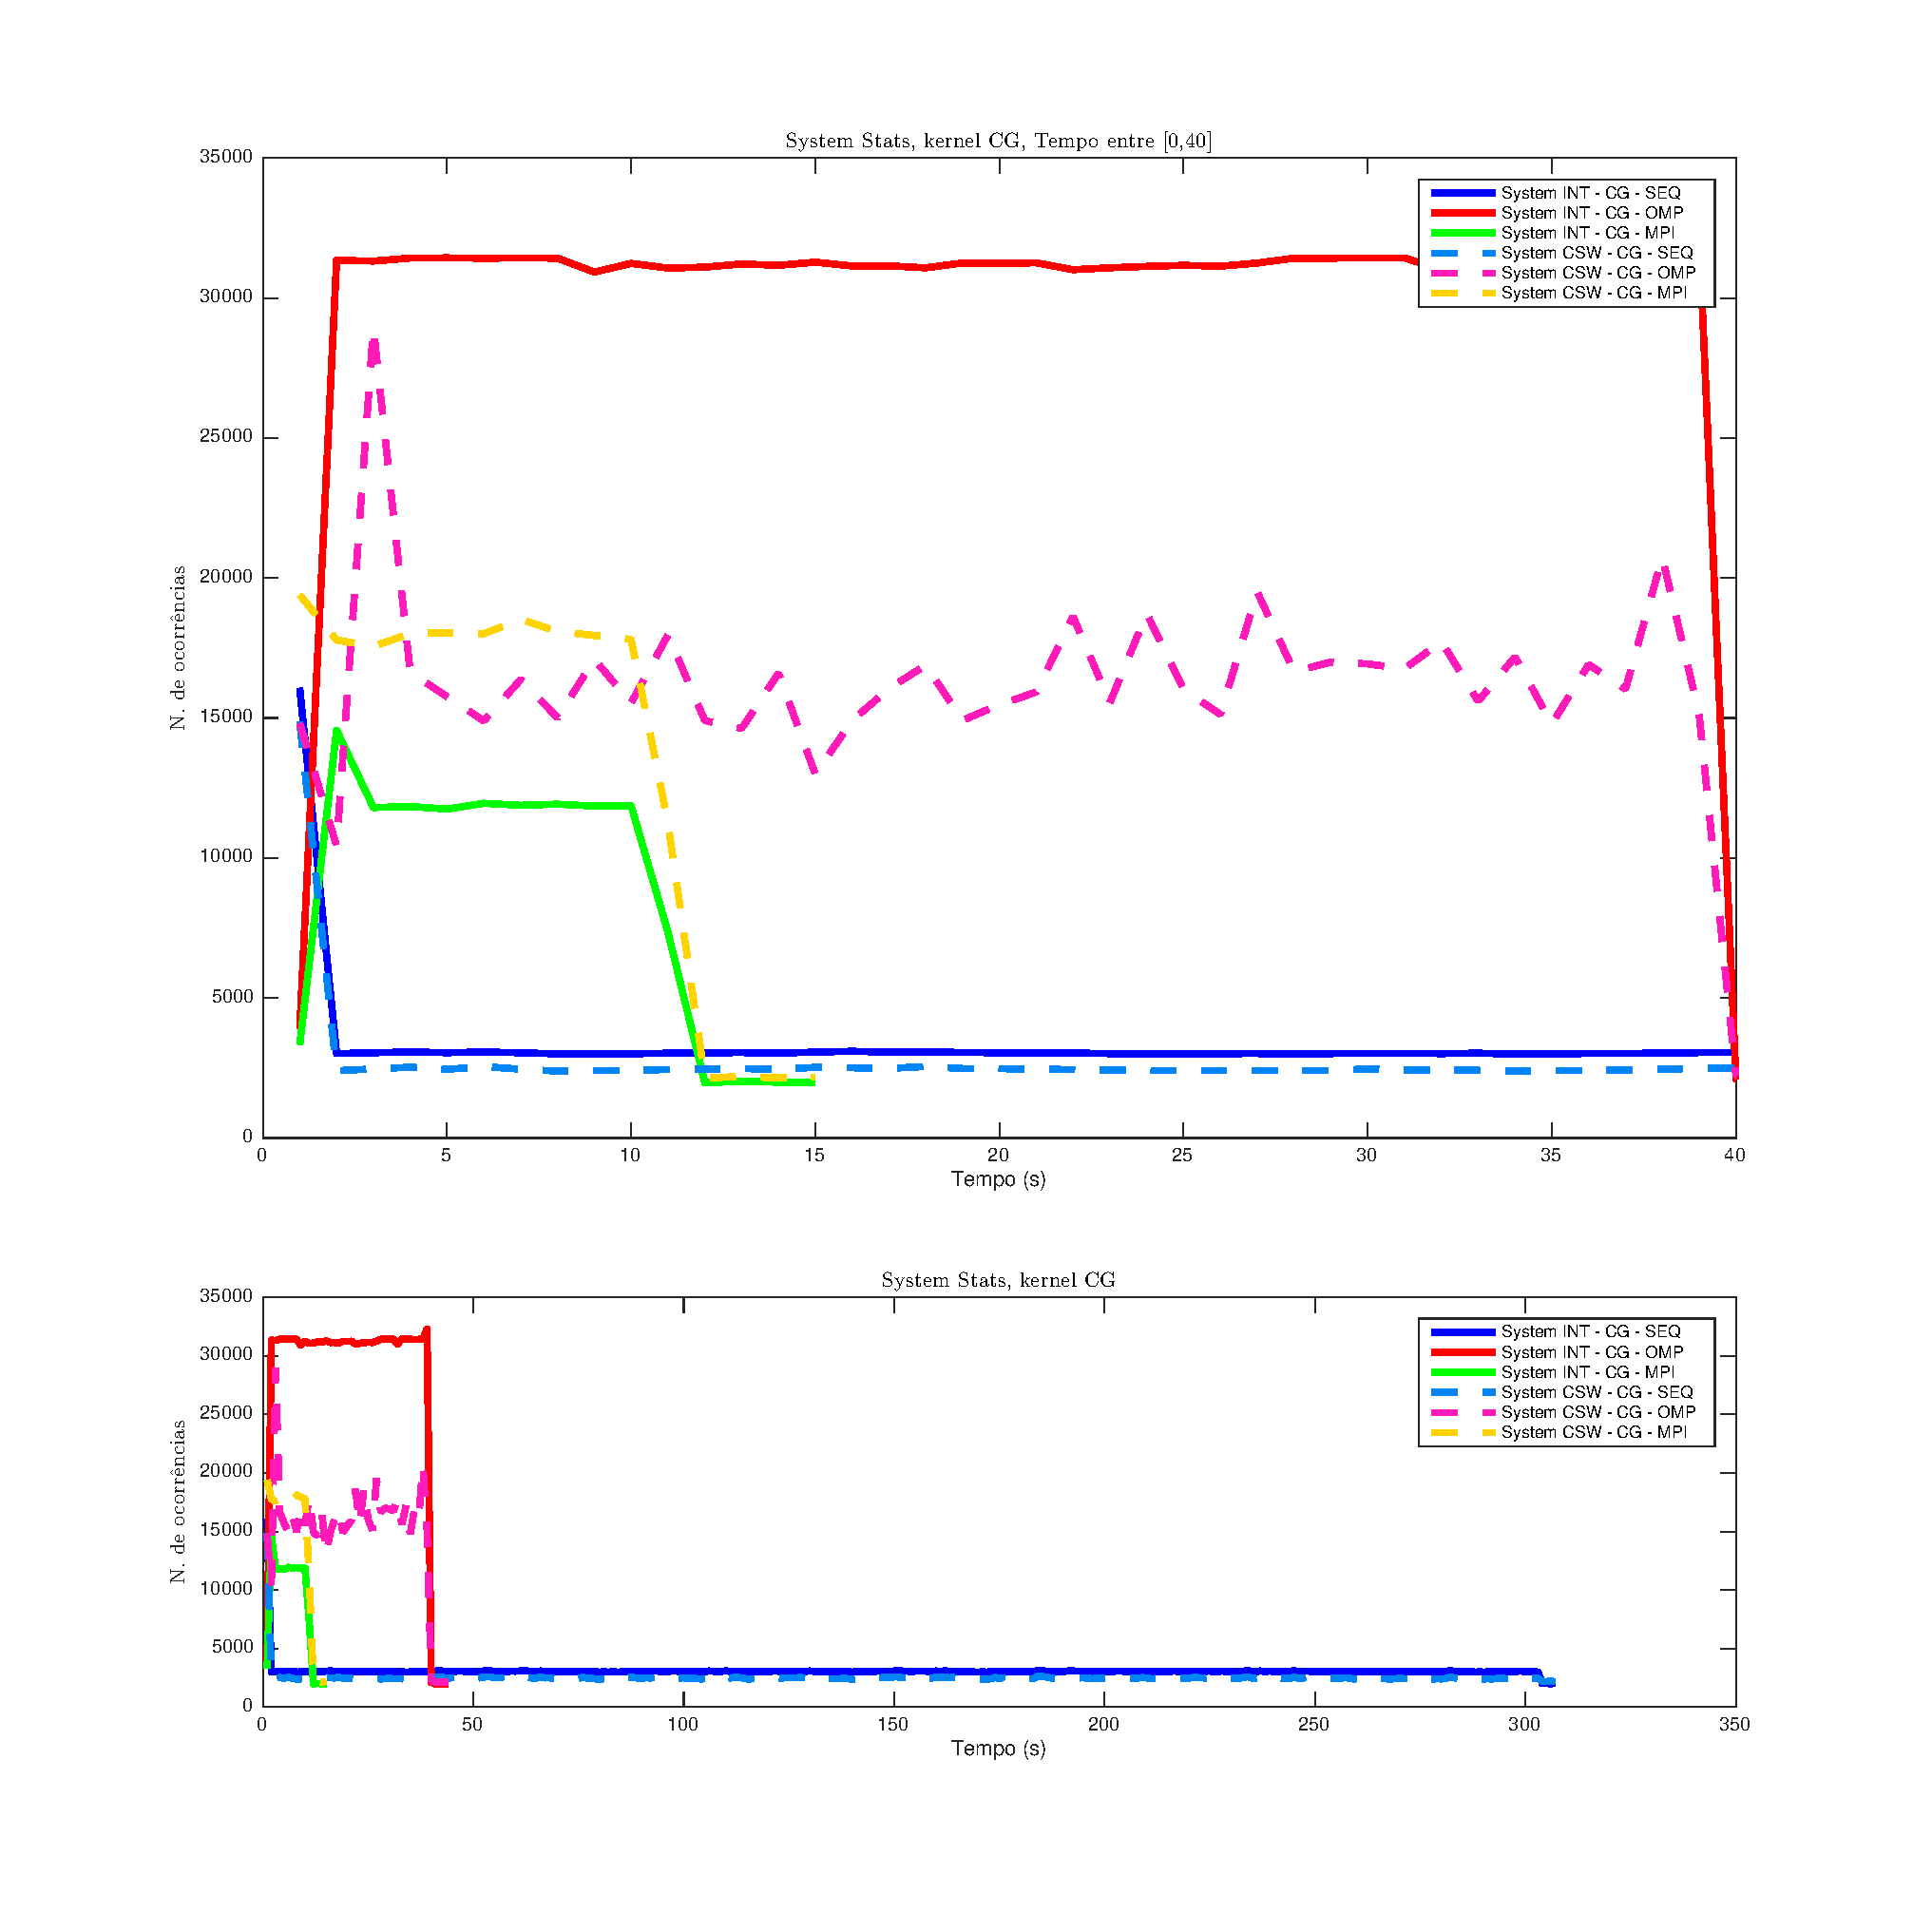
\includegraphics[width=0.9\columnwidth]{EPS/dstat_CG_seq_vs_omp_vs_mpi/system.eps}
\caption{\tiny Relação de número de interrupções de processo e número de "context swap" para os kernels SEQ/OMP/MPI - CG, nós 641, classe de dados C para compilador gcc 4.9.0 com flag de compilação  -O3, para comunicação Myrinet 10Gbps (memória distribuída)}
\label{dstat_cg_SOM_system}
\end{figure}
\end{columns}

\end{frame}


\begin{frame}
  \titlepage
\end{frame}

  
\end{document}




